\section{Définitions et quelques résultats préliminaire}

% \subsection{Développement en fraction continue de $C(z)$}
% % \subsection{Nombres de Catalan}
% % \subsection{Fractions continues de Stieltjes}
% % \subsection{Fonction génératrice ordinaire des nombres de Fine}
% % \subsection{Relation de récurrence entre $C_{n}$ et $F_{n}$}
% % \subsection{Bijection entre $\mathcal{F}_{n}$ et $\overline{\rm{Dyck}}$$(n)$}

\subsection{Fraction continues}
\begin{frame}[allowframebreaks]{S-Fraction et J-Fraction}
    \transfade
    \begin{block}{S-Fraction}
        Une S-fraction est une expression de la forme:\\
        \[
			S(z)=\cfrac{1}{1-\cfrac{c_{1}z}{1-\cfrac{c_{2}z}{1-\cfrac{c_{3}z}{\ddots}}}}
		\]
    \end{block}

    \begin{block}{J-Fraction}
        Une J-fraction est une expression de la forme:\\
        \[
			J(z)=\cfrac{1}{1-c_{1}z-\cfrac{c_{1}c_{2}z^2}{1-(c_{2}+c_{3})z-\cfrac{c_{3}c_{4}z^2}{1-(c_{4}+c_{5})z-\cfrac{c_{5}c_{6}z^2}{\ddots}}}}  
		\]
        D'après le Lemme 2.11 de \cite{9}, on a $S(z)=J(z)$
    \end{block}
\end{frame}



\subsection{Nombres de Catalan}
\begin{frame}{Nombres de Catalan}
    \transfade
    \begin{block}<1->{Définition}
        Le nombre de Catalan d'ordre $n\geq 1$ est défini par \\
        \begin{rm}
            \begin{itemize}
                \item [($i$)] $C_{0}=1$
                \item [($ii$)] $\forall n \geq 1$, $C_{n} = \underset{i=0}{\overset{n-1}{\sum}}C_{i}C_{n-i-1}$
            \end{itemize}
        \end{rm}
    \end{block}

    \begin{block}<2->{Développement en fraction continue de la fgo}
        \begin{rm}
            On a $C(z) = \cfrac{1}{1-z-\cfrac{z^2}{1-2z-\cfrac{z^2}{\ddots}}} $\\
        \end{rm}
        où $C(z)=\sum\limits_{n\geq 0}C_{n}z^{n}$
    \end{block}
\end{frame}



\subsection{Chemins de Motzkin}
\begin{frame}{Définition de quelques chemins}
    \transfade
    \begin{block}<1->{Chemins de Motzkin}
        \begin{rm}
            Les chemins de Motzkin sont les éléments de l'ensemble $\Gamma_{n,1}^{0}$ qui vérifient, pour tout $c \in \Gamma_{n,1}^{0}$:
            \begin{itemize}
                \item[$(i)$] $\forall i \in [n]$, $|c_{1}c_{2}\cdots c_{i}|_{m} \geq |c_{1}c_{2}\cdots c_{i}|_{d} $
                \item[$(ii)$] $|c_{1}c_{2}\cdots c_{n}|_{m} = |c_{1}c_{2}\cdots c_{n}|_{d} $
            \end{itemize}
        \end{rm}
    \end{block}
    
    % \begin{block}<2->{2-Chemins de Motzkin}
    %     Un 2-chemin de Motzkin est un chemin de Motzkin caractérisé par deux types de paliers : le palier rouge, noté $r$, et le palier bleu, noté $b$. De plus, un chemin $c = c_{1}c_{2}\cdots c_{n}$, avec $c_{k} \in \{m, d, r, b\}$, est considéré comme un 2-chemin de Motzkin s'il ne comporte aucun palier rouge de niveau zéro.
    % \end{block}
\end{frame}

\begin{frame}
    \begin{block}{2-Chemins de Motzkin}
        Un 2-chemin de Motzkin est un chemin de Motzkin caractérisé par deux types de paliers : le palier rouge, noté $r$, et le palier bleu, noté $b$. De plus, un chemin $c = c_{1}c_{2}\cdots c_{n}$, avec $c_{k} \in \{m, d, r, b\}$, est considéré comme un 2-chemin de Motzkin s'il ne comporte aucun palier rouge de niveau zéro.
    \end{block}
    \begin{figure}
        \centering
        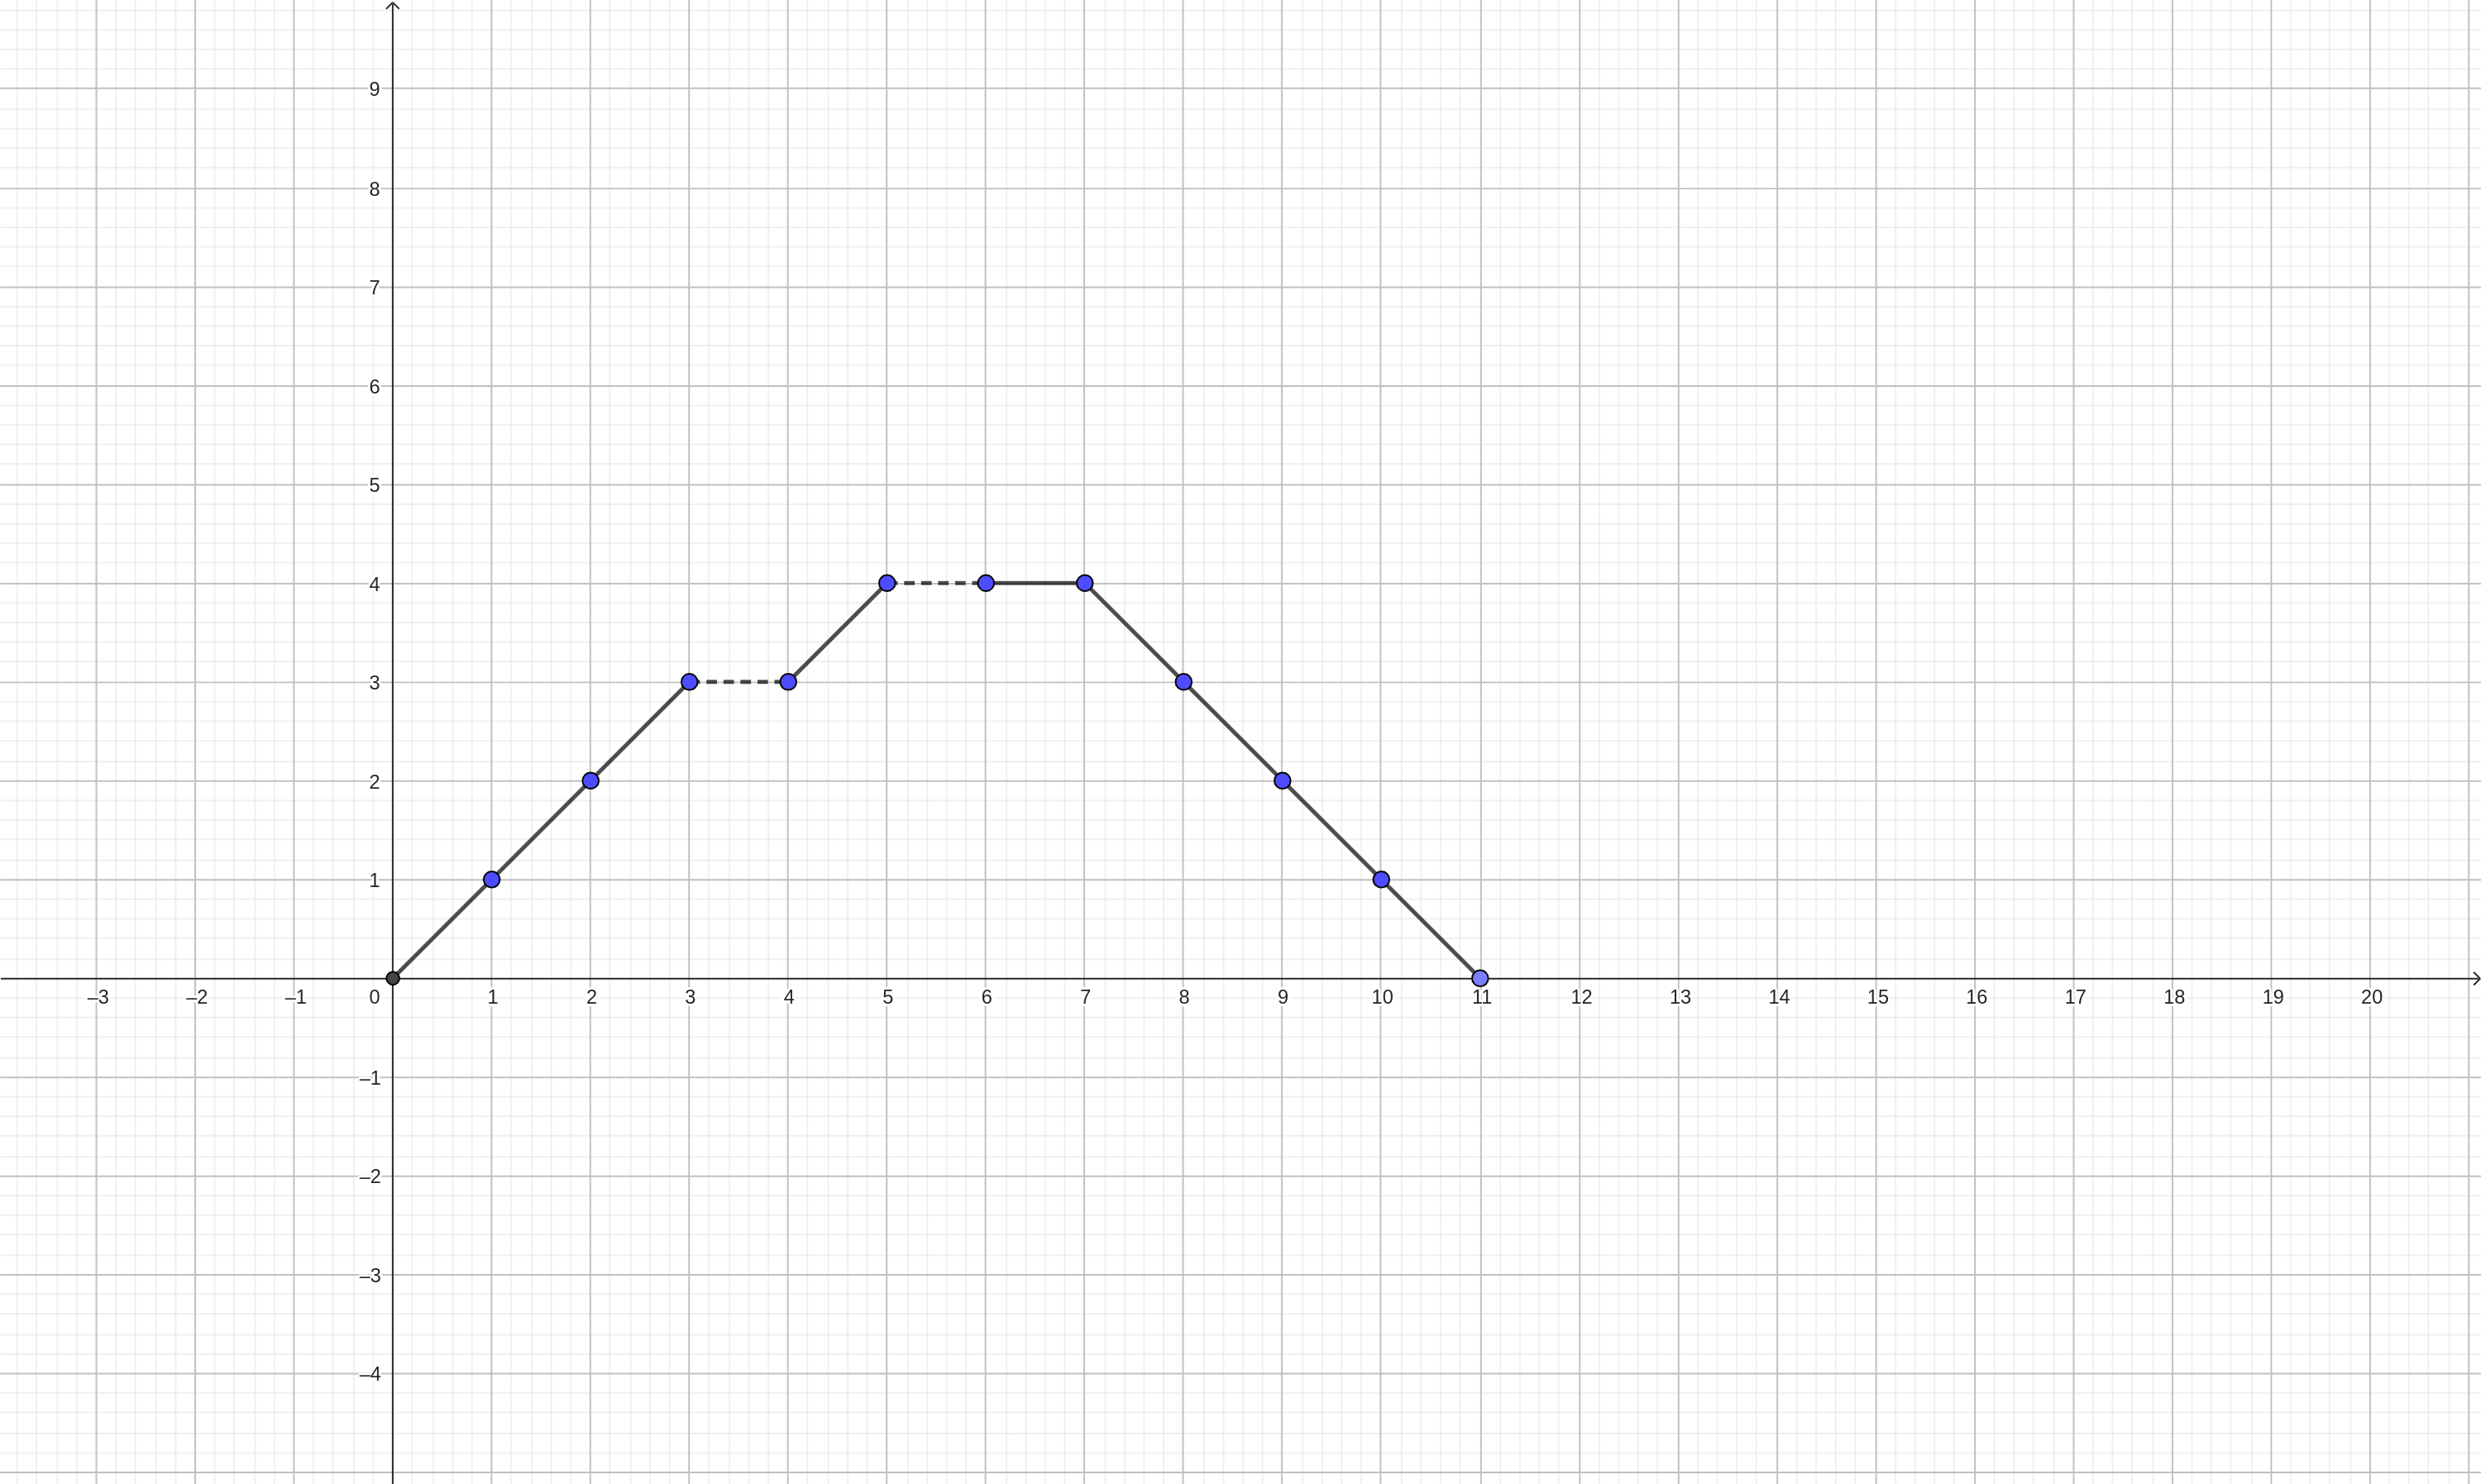
\includegraphics[width=0.7\textwidth]{./images/2-chemin Motzkin.png}
        \caption{2-Chemin de Motzkin}
        \label{fig:example}
      \end{figure}
\end{frame}

\begin{frame}{Définition de quelques chemins}
    \transfade
    \begin{block}<1->{Chemins de Motzkin valués}
            Un 2-chemin de Motzkin valué est un couple (c,p) où $c = c_{1}c_{2}\cdots c_{n}$\\ et $p = p_{1}p_{2}\cdots p_{n}$
            vérifient les conditions suivantes:
            \begin{itemize}
                \item$c \in \Gamma_{n}$
                % \item[$(ii)$.] p est le poids associé à c
                \item$0\leq p_{i}\leq \gamma_{i-1}$, si $c_{i}=m\text{ ou }c_{i}=b$
                \item $0\leq p_{i}\leq \gamma_{i-1} - 1$, si  $c_{i}=d\text{ ou }c_{i}=r$
            \end{itemize}
    \end{block}
\end{frame}

\begin{frame}[t]{Quelques résultats sur les chemins}
    \begin{block}<1->{Proposition}
        La J-fraction des $(|\Gamma_{n}|)$ est $\Gamma(z) = \cfrac{1}{1-z-\cfrac{z^2}{1-2z-\cfrac{z^2}{\ddots}}}$\\
        \vspace{7pt} où $\Gamma(z)=1+\sum\limits_{n\geq 1}|\Gamma_{n}|z^n$
    \end{block}

    \begin{block}<2->{Corollaire}
        On a $|\Gamma_{n}|=C_{n}$
    \end{block}
\end{frame}


\subsection{Chemins de Fine}
\begin{frame}[t]{Premier aperçu sur les nombres de Fine}
    \transfade
    \begin{block}<1->{Définition}
        Un chemin de Fine est un 2-chemin de Motzkin sans palier bleu de niveau zéro. On note par $\mathcal{F}_{n}$ l'ensemble de tels chemins
    \end{block}
    
    \begin{block}<2->{Proposition}
        On a $F(z)=\cfrac{1}{1-\cfrac{z^2}{1-2z-\cfrac{z^2}{\ddots}}} = \cfrac{1}{2+z}(1+C(z))$\\ 
        \vspace{7pt} où $F(z)=\sum\limits_{n\geq 0}F_{n}z^n$ et $F_{n}=|\mathcal{F}_{n}|$
    \end{block}
\end{frame}

\begin{frame}
    \frametitle{Quelques relations de récurrence}
    \transfade
    \begin{center}
        \begin{itemize}
            \item $[z^{n}]C(z) = C_{n} = 2F_{n} + F_{n-1}, (n\geq 1)$
            \pause
            \item $[z^n]F(z) = F_{n} = \cfrac{1}{2}\sum\limits_{k=0}^{n-2}(-\cfrac{1}{2})^{k}C_{n-k}, (n\geq 2)$
            \pause
        \end{itemize}
    \end{center}
\end{frame}

\begin{frame}
    % La proposition suivante nous a permis d'en déduire la dernière relation des relations précédentes.
    \transfade
    \begin{block}{Proposition 1}
        La transformation $\theta: \mathcal{F}_{n} \longrightarrow  \overline{\rm{Dyck}}(n)$; $c \longrightarrow p=p_{1}\cdots p_{2n}$ définie comme suit, pour tout $i \in [n]$,
        $$
            p_{2i-1}p_{2i}=\begin{cases}
                mm & \text{ si } c_{i}=m \\
                dd & \text{ si } c_{i}=d \\
                md & \text{ si } c_{i}=b \\
                dm & \text{ si } c_{i}=r \\
            \end{cases}
        $$
        est une application bijective où $\overline{\text{Dyck}}(n)$ l'ensemble des chemins de Dyck qui
        vérifient la condition si $p_{i}=m \text{ et } \gamma_{i-1}=0$, alors  $p_{i+1}=m$.
    \end{block}
    \pause
    \begin{block}{Proposition 2}
        On a $F_{n}=\sum\limits_{k=2}^{n}C_{k-1}F_{n-k}$
    \end{block}
\end{frame}


